\documentclass[a4paper,11pt]{article}

\usepackage{graphicx} % Required for inserting images
\usepackage[english,greek]{babel}
\usepackage[utf8x]{inputenc}
\usepackage{amsmath}
\usepackage{multirow}
\usepackage{enumitem}
\usepackage{graphicx}
\usepackage{subcaption}
\usepackage{float}
\usepackage{array}
\usepackage{changepage}
\usepackage[nottoc]{tocbibind}


\graphicspath{images/}

\newcommand{\lt}{\latintext}
\newcommand{\gt}{\greektext}

\setlength{\arrayrulewidth}{0.3mm}
\setlength{\tabcolsep}{8pt}
\renewcommand{\arraystretch}{1.5}

\title{Δεύτερη υποχρεωτική εργασία στην Αριθμητική Ανάλυση}
\author{\gt Ονοματεπώνυμο: Νικόλαος Αργυρίου \\  ΑΕΜ: 4367}
\date{\today}

\begin{document}

\maketitle

\setcounter{section}{4}
\section{Άσκηση 5}
\subsection{Εισαγωγή}

\gt Ο κώδικας για την άσκηση βρίσκεται στον φάκελο \lt ask5.

\gt Σε αυτήν την άσκηση θα προσεγγιστεί με τρεις διαφορετικές μεθόδους η συνάρτηση του ημιτόνου στο διάστημα \lt \([-\pi, \pi]\). \gt Για τις προσεγγίσεις χρησιμοποιούνται τα εξής ανομοιόμορφα κατανεμημένα σημεία του καρτεσιανού επιπέδου, τα οποία ικανοποιούν τη συνάρτηση του ημιτόνου όμως με ακρίβεια πέντε δεκαδικών ψηφίων:

\begin{itemize}
\item $(-\pi, 0)$ \item $(-2.5, -0.59847)$ \item $(-\pi/2, -1)$ \item $(-1.4, -0.98544)$ \item $(-0.6, -0.56464)$ \item $(0, 0)$ \item $(1, 0.84147)$ \item
$(\pi/2, 1)$ \item $(2.7, 0.42737)$ \item $(\pi, 0)$
\end{itemize}

\subsection{\gt Πολυωνυμική προσέγγιση}

Ο κώδικας βρίσκεται στο αρχείο \lt ask5a.py \gt Για την προσέγγιση επιλέχθηκε το πολυώνυμο \lt Lagrange. \gt Η συνάρτηση που υλοποιεί τη μέθοδο \lt \verb|lagrange_polynomial| \gt δέχεται ένα σύνολο σημείων, το διατρέχει και κάθε φορά προσθέτει στο πολυώνυμο την ποσότητα $yL(x)$, όπου $L(x)$ είναι ο συντελεστής \lt Lagrange \gt που έχει υπολογιστεί για ένα συγκεκριμένο σημείο. Παρακάτω παρουσιάζεται το σφάλμα της μεθόδου.

\begin{figure}[h!]
    \centering
    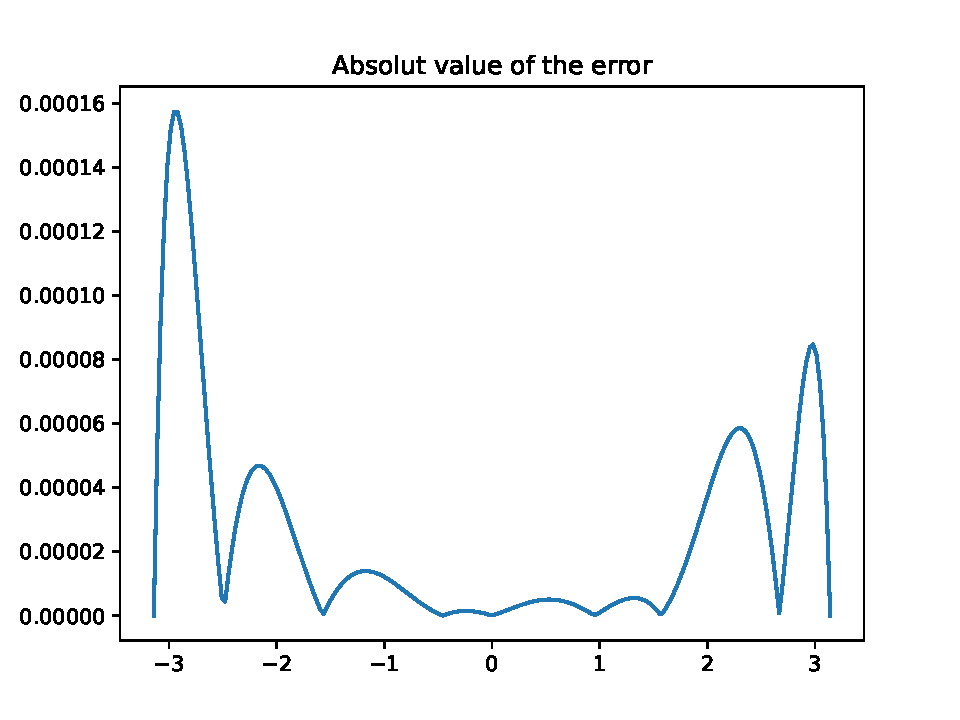
\includegraphics[width=0.8\linewidth]{images/figure5a.pdf}
    \centering
     \caption{Η απόλυτη τιμή του σφάλματος του πολυωνύμου \lt Lagrange}
    \label{fig:fig5a}
\end{figure}

\begin{table}[h]
\centering
\label{fig:table5a}
\begin{tabular}{c c c}
   \gt & Απόλυτη τιμή σφάλματος & Ψηφία ακρίβειας \\
   Ελάχιστη τιμή & 0.0000000000002650 & 12 \\
   Μέγιστη τιμή & 0.0001574509618303 & 3 \\
   Μέση τιμή & 0.0000259359207534 & 4 \\
\end{tabular}
\caption{\gt Σφάλμα του πολυώνυμου \lt Lagrange}
\end{table}

\subsection{\lt Splines}

Ο κώδικας βρίσκεται στο αρχείο \lt ask5b.py \gt Η συνάρτηση \lt \verb|get_splines| \gt δέχεται τα σημεία και επιστρέφει μια λίστα που περιέχει τα πολυώνυμα των φυσικών κυβικών \lt splines. \gt Αν τα σημεία είναι \lt n+1 \gt τότε ο αριθμός των \lt splines \gt είναι \lt n. \gt Κάθε \lt spline \gt ορίζεται ως $s^{(i)}(x)=\alpha_0^{(i)}+\alpha_1^{(i)}x+\alpha_2^{(i)}x^2+\alpha_3^{(i)}x^3$ και για τον υπλογισμό τους χρησιμοποιούνται οι εξής εξισώσεις:

\begin{itemize}
\item $s^{(i)}(x_i)=f(x_i), i=0, ..., n-1$
\item $s^{(i)}(x_{i+1})=f(x_{i+1}), i=0, ..., n-1$
\item $(s^{(i-1)})'(x_{i})=(s^{(i)})'(x_i), i=1, ..., n-1$
\item $(s^{(i-1)})''(x_{i})=(s^{(i)})''(x_i), i=1, ..., n-1$
\item $(s^{(0)})''(x_0)=(s^{(n)})''(x_n)=0$
\end{itemize}

Η επίλυση των παραπάνω εξισώσεων ανάγεται στην επίλυση ενός γραμμικού συστήματος $Ax = b$. Κάθε γραμμή του πίνακα Α εκφράζει και μία διαφορετική εξίσωση, ενώ το διάνυσμα $x$ αντιπροσωπεύει τον τύπο των \lt splines \gt ανά τέσσερις συντεταγμένες ($x_0=\alpha_0^{(0)}$, $x_1=\alpha_1^{(0)}$, ..., $x_4=\alpha_0^{(1)}$, ...). Αφού υπολογίσουμε τα \lt n \gt πολυώνυμα, λαμβάνουμε τα παρακάτω σφάλματα.

\begin{figure}[h!]
    \centering
    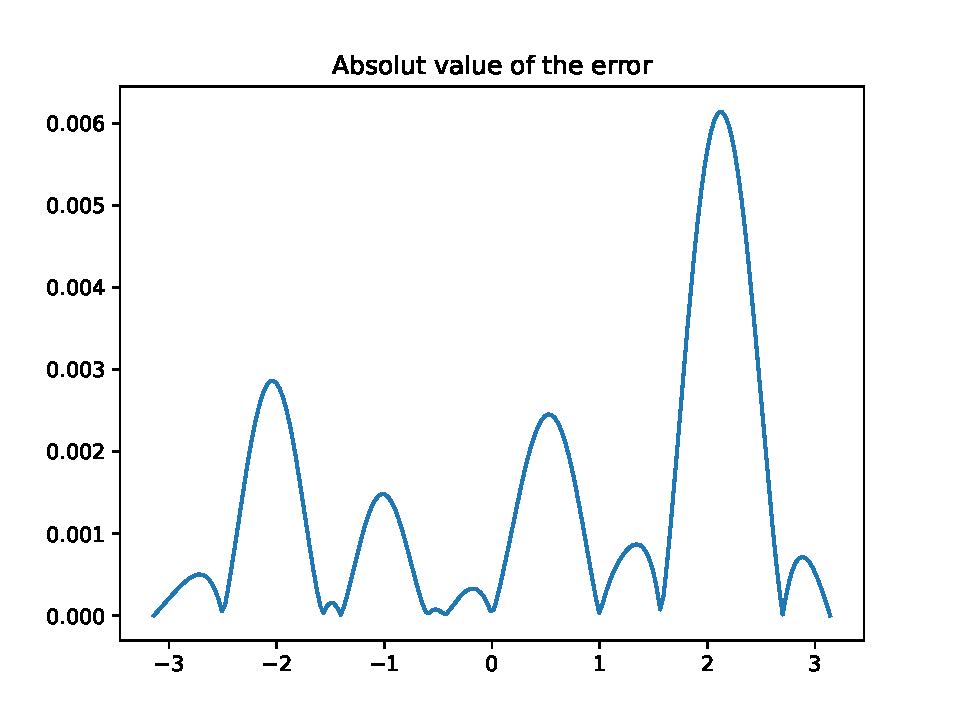
\includegraphics[width=0.8\linewidth]{images/figure5b.pdf}
    \centering
     \caption{Η απόλυτη τιμή του σφάλματος των \lt splines}
    \label{fig:fig5b}
\end{figure}

\begin{table}[h]
\centering
\label{fig:table5b}
\begin{tabular}{c c c}
   \gt & Απόλυτη τιμή σφάλματος & Ψηφία ακρίβειας \\
   Ελάχιστη τιμή & 0.0000000000000012 & 14 \\
   Μέγιστη τιμή & 0.0061455725161046 & 1 \\
   Μέση τιμή & 0.0013744890469981 & 2 \\
\end{tabular}
\caption{\gt Σφάλμα των \lt splines}
\end{table}

\subsection{\gt Μέθοδος ελαχίστων τετραγώνων}

Ο κώδικας βρίσκεται στο αρχείο \lt ask5c.py \gt Η συνάρτηση \lt \verb|least_squares_method| \gt δέχεται τα αρχικά σημεία και τον βαθμό του πολυωνύμου προσέγγισης και επιστρέφει το υπολογισμένο πολυώνυμο προσέγγισης, καθώς και τη δεύτερη νόρμα του διανύσματος υπολοίπων $r$. Το πολυώνυμο είναι της μορφής $y=\alpha_{0}+\alpha_{1}x+\dots+\alpha_{k}x^{k}$. Για κάθε σημείο $(x_i, y_i)$ αντικαθιστούμε τις συντεταγμένες του στην προηγούμενη εξίσωση και έτσι σχηματίζεται το γραμμικό σύστημα $Ax=b$ μορφής
\[
    \begin{bmatrix}
        1 & x_0 & x_0^2 & \dots & x_0^k \\
        1 & x_1 & x_1^2 & \dots & x_1^k \\
        \vdots & \vdots & \vdots & \vdots & \vdots \\
        1 & x_{n+1} & x_{n+1}^2 & \dots & x_{n+1}^k \\
    \end{bmatrix}
    \begin{bmatrix}
        \alpha_{0} \\
        \alpha_{1} \\
        \vdots \\
        \alpha_{k}
    \end{bmatrix}
    =
    \begin{bmatrix}
        y_{0} \\
        y_{1} \\
        \vdots \\
        y_{k}
    \end{bmatrix}
\]

Επειδή οι εξισώσεις είναι περισσότερες από τους αγνώστους, το σύστημα είναι αδύνατο. Συνεπώς πολλαπλασιάζουμε από αριστερά τα δύο μέλη της εξίσωσης με $A^T$ και τώρα έχουμε να λύσουμε το σύστημα $Cx=d$, όπου $C=A^TA$ και $d=A^Tb$. Το διάνυσμα λύσης $x$ μάς δίνει το πολυώνυμο ελαχίστων τετραγώνων.

Στο συγκεκριμένο πρόβλημα επιλέγεται πολυώνυμο ογδόου βαθμού, για το οποίο η νόρμα του διανύσματος υπολοίπου είναι 0.0000837543727750. Τα σφάλματα παροουσιάζονται στο σχήμα \ref{fig:fig5c} στον πίνακα \ref{fig:table5c}.

\begin{figure}[h!]
    \centering
    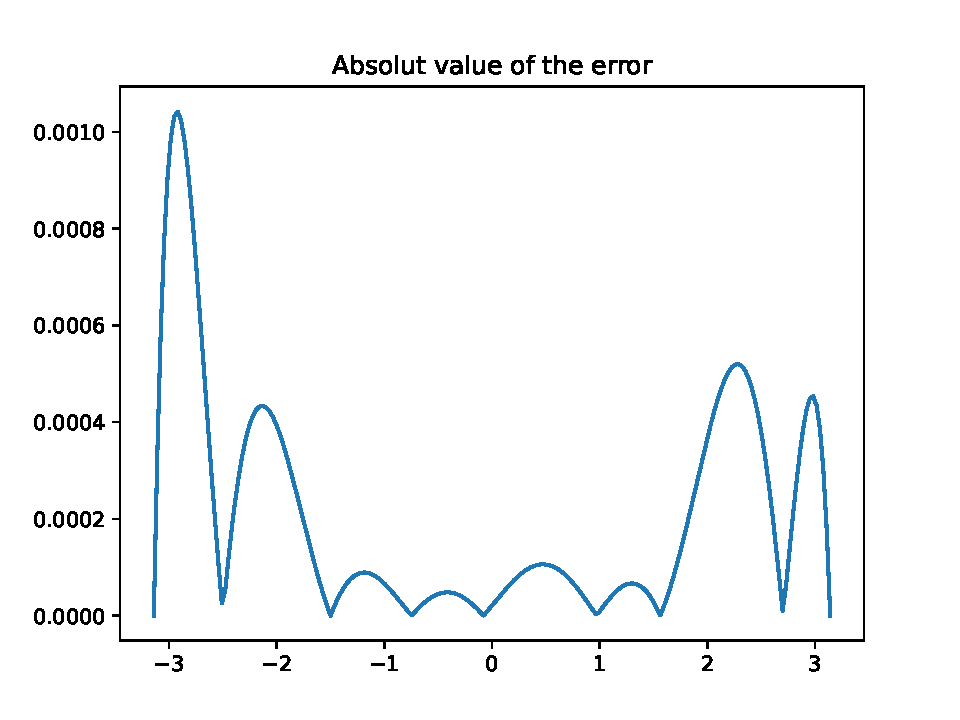
\includegraphics[width=0.8\linewidth]{images/figure5c.pdf}
    \centering
     \caption{Η απόλυτη τιμή του σφάλματος του πολυωνύμου ελαχίστων τετραγώνων}
    \label{fig:fig5c}
\end{figure}

\begin{table}[ht]
\centering
\begin{tabular}{c c c}
   \gt & Απόλυτη τιμή σφάλματος & Ψηφία ακρίβειας \\
   Ελάχιστη τιμή & 0.0000000115053708 & 7 \\
   Μέγιστη τιμή & 0.0010420414431526 & 2 \\
   Μέση τιμή & 0.0002067383707707 & 3 \\
\end{tabular}
\caption{\gt Σφάλμα του πολυωνύμου ελαχίστων τετραγώνων}
\label{fig:table5c}
\end{table}

\subsection{Συμπεράσματα}

Από την ανάλυση που έχουμε κάνει συμπεραίνουμε ότι η μέθοδος του \lt Lagrange \gt παρουσιάζει καλύτερη μέση ακρίβεια από τις άλλες δύο πετυχαίνοντας τέσσερα δεκαδικά ψηφία. Όσον αφορά τη μέγιστη τιμή του σφάλματος, το πολυώνυμο \lt Lagrange \gt και πάλι λαμβάνει την πρώτη θέση έχοντας το μικρότερο σφάλμα (0.0001574509618303) και τρία ψηφία ακρίβειας. Όμως οι \lt splines \gt έχουν το μικρότερο ελάχιστο σφάλμα (0.0000000000000012) με 14 ψηφία ακρίβειας. Επομένως ενώ αρχικά επιθυμούσαμε ακρίβεια πέντε δεκαδικών ψηφίων, τελικά πετύχαμε με τη μέθοδο \lt Lagrange \gt μία μέση ακρίβεια τεσσάρων ψηφίων.

\section{Άσκηση 6}
\subsection{Εισαγωγή}

\gt Ο κώδικας για την άσκηση βρίσκεται στον φάκελο \lt ask6.

\gt Σε αυτήν την άσκηση θα υπολογιστεί με δύο διαφορετικές μεθόδους το ολοκλήρωμα $\int_0^{\frac{\pi}{2}}sin(x)dx$. Σε κάθε περίπτωση επιλέγονται έντεκα σημεία του διάστηματος $[0, \pi/2]$, τέτοια ώστε να δημιουργούνται δέκα ομοιόμορφα κατανεμημένοι διαμερισμοί του διαστήματος. 

Ας σημειώσουμε εδώ ότι λύνοντας το παραπάνω ολοκλήρωμα με την αναλυτική μαθηματική μέθοδο παίρνουμε την τιμή 1.

\subsection{Μέθοδος \lt Simpson}

\gt Η συνάρτηση που υλοποιεί τη μέθοδο βρίσκεται στο αρχείο \lt ask6a.py \gt και ονομάζεται \lt \verb|simpson_method|. \gt Δέχεται τη συνάρτηση \lt f \gt του ολοκληρώματος, το κάτω \lt a \gt και το άνω \lt b \gt όριό του, καθώς και τον αριθμό των διαμερισμών \lt N \gt που θέλουμε να γίνουν και επιστρέφει την προσεγγιστική τιμή του ολοκληρώματος. Ο υπολογισμός γίνεται μέσω του τύπου 
\[\int_a^bf(x)dx \simeq \frac{b-a}{3N} \Big(f(x_0) +f(x_N) + 2\sum_{i=1}^{\frac{N}{2}-1}f(x_{2i}) + 
4\sum_{i=1}^{\frac{N}{2}}f(x_{2i-1})\Big)\]

Αν τρέξουμε το πρόγραμμα λαμβάνουμε την τιμή 1.0000033922209004. Η αριθμητική τιμή του σφάλματος της μεθόδου \lt Simpson \gt είναι 1 - 1.0000033922209004 = $-3.3922209004 \times 10^{-6}$. Αυτό το σφάλμα βρίσκεται ανάμεσα στα θεωρητικά όρια:
\[|\verb|σφάλμα|| \leq \frac{(b-a)^5}{180N^4}M,\] 
\[\verb|όπου |M=max\{|f^{(4)}(x)|:x\in[a, b]\}=max\{|\sin{x}|:x\in[0,\frac{\pi}{2}]\}=1\]
Συνεπώς έχουμε:
\[|\verb|σφάλμα|| \leq \frac{(\frac{\pi}{2}-0)^5}{180\times10^4}\times1 = \frac{\frac{\pi^5}{32}}{1800000} \simeq 5.31284\times10^{-6}\]

\subsection{Μέθοδος τραπεζίου}

Η μέθοδος του τραπεζίου υλοποιείται από τη συνάρτηση \lt \verb|trapezoid_method| \gt στο αρχείο \lt ask6b.py \gt Ως ορίσματα δέχεται τη συνάρτηση \lt f \gt του ολοκληρώματος, το κάτω \lt a \gt και το άνω \lt b \gt όριό του και τον αριθμό των διαμερισμών \lt N \gt που θέλουμε να γίνουν και επιστρέφει την προσεγγιστική τιμή του ολοκληρώματος. Ο χρησιμοποιούμενος τύπος είναι 
\[\int_a^bf(x)dx \simeq \frac{b-a}{2N} \Big(f(x_0) +f(x_N) + 2\sum_{i=1}^{N-1}f(x_{i})\Big)\]

Με 10+1 σημεία η συνάρτηση μάς δίνει την προσεγγιστική τιμή \newline 0.9979429863543572. Το αριθμητικό σφάλμα είναι 1 - 0.9979429863543572 = $2.0570136456428 \times 10^{-3}$, το οποίο επαληθεύει το θεωρητικό σφάλμα:

\[|\verb|σφάλμα|| \leq \frac{(b-a)^3}{12N^2}M,\] 
\[\verb|όπου |M=max\{|f''(x)|:x\in[a, b]\}=max\{|-\sin{x}|:x\in[0,\frac{\pi}{2}]\}=1\]
Συνεπώς έχουμε:
\[|\verb|σφάλμα|| \leq \frac{(\frac{\pi}{2}-0)^3}{12\times10^2}\times1 = \frac{\frac{\pi^3}{8}}{1200} \simeq 3.22982\times10^{-3}\]

\section{Άσκηση 7}
\subsection{Εισαγωγή}

\gt Ο κώδικας για την άσκηση βρίσκεται στον φάκελο \lt ask7. \gt Στην άσκηση αυτή θα κάνουμε πρόβλεψη της τιμής μετοχών δύο διαφορετικών εταιριών, της ΔΕΗ και του ΟΤΕ, χρησιμοποιώντας τη μέθοδο ελαχίστων τετραγώνων, η οποία υλοποιήθηκε σε προηγούμενη άσκηση. Σε κάθε περίπτωση οι εκτιμήσεις γίνονται με βάση τις τιμές κλεισίματος δέκα ημερών (ημέρες 0-9) και στη συνέχεια γίνεται πρόβλεψη της τιμής για τις ημέρες 11 και 15 με πολυώνυμα δευτέρου, τρίτου και τέταρτου βαθμού. 

\subsection{Πρόβλεψη τιμής μετοχής της ΔΕΗ}

\begin{figure}[h!]
    \centering
    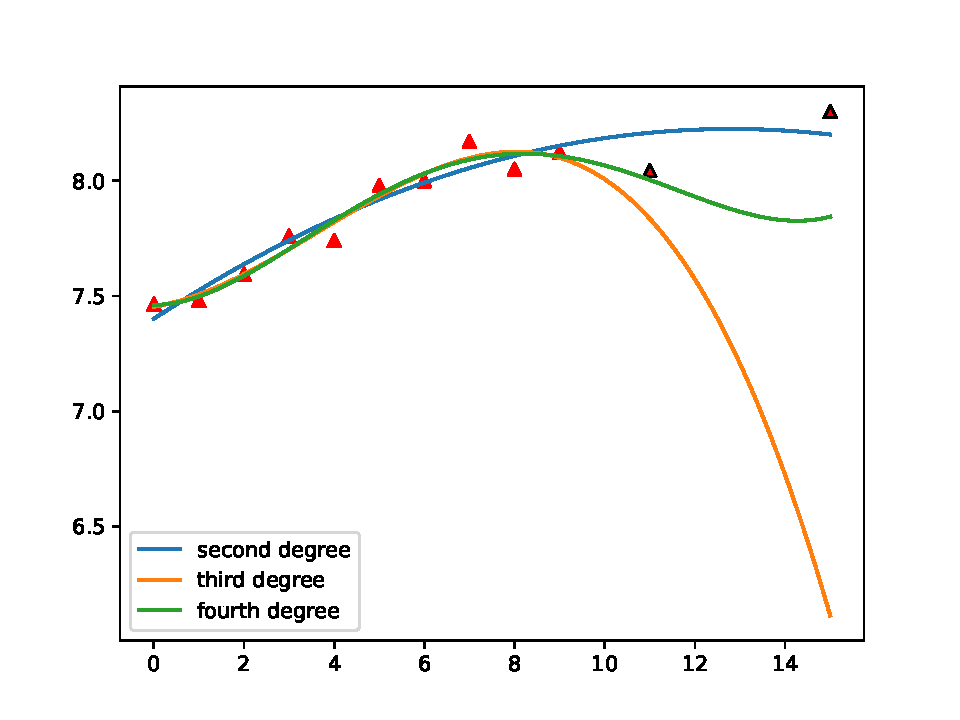
\includegraphics[width=0.8\linewidth]{images/figure7_dei.pdf}
    \centering
     \caption{Οι τιμές της μετοχής και η εκτίμησή τους}
    \label{fig:fig7dei}
\end{figure}

\begin{table}[ht]
\centering
\begin{tabular}{c c| c c c}
    & & \multicolumn{3}{c}{Πολυώνυμα} \\
   Ημέρα & Πραγματική τιμή & Δευτεροβάθμιο & Τριτοβάθμιο & Τεταρτοβάθμιο \\
   11 (21-2) & 8.045 & 8.2081136 & 7.8350606 & 8.003447 \\
   15 (28-2) & 8.3 & 8.2005227 & 6.1131725 & 7.8442512 \\
\end{tabular}
\caption{Οι προβλέψεις τιμών για τις δύο συνεδριάσεις}
\label{fig:table7a}
\end{table}

\begin{table}[h!]
\centering
\begin{tabular}{c c c c}
    & \multicolumn{3}{c}{Πολυώνυμα} \\
   Ημέρες & Δευτεροβάθμιο & Τριτοβάθμιο & Τεταρτοβάθμιο \\
   0-9 & 0.0534894 & 0.0426487 & 0.0407267 \\
   11 (21-2) & 0.1631136 & 0.2099394 & 0.0415530 \\
   15 (28-2) & 0.0994773 & 2.1868275 & 0.4557488 \\
\end{tabular}
\caption{Σφάλματα των προσεγγίσεων}
\label{fig:table7b}
\end{table}

Στο σχήμα \ref{fig:fig7dei} απεικονίζονται οι τρεις πολυωνυμικές προσεγγίσεις (δευτέρου, τρίτου και τετάρτου βαθμού), καθώς και οι πραγματικές τιμές της μετοχής για τις ημέρες 0 έως 9, 11 και 15. Ο πίνακας \ref{fig:table7a} παρουσιάζει ακριβώς τις εκτιμήσεις για τις δύο ημέρες που μας ενδιαφέρουν, ενώ ο πίνακας \ref{fig:table7b} δείχνει την απόλυτη τιμή των σφαλμάτων.  Βλέπουμε ότι για τις πρώτες δέκα ημέρες οι προσεγγίσεις ακολουθούν με αρκετά καλό τρόπο τις πραγματικές τιμές. Η καλύτερη εκτίμηση για την 21η Φεβρουαρίου 2023 είναι αυτή μέσω του τεταρτοβάθμιου πολυωνύμου, ενώ για την 28η Φεβρουαρίου είναι αυτή μέσω του δευτεροβάθμιου πολυωνύμου. Ας σημειώσουμε εδώ ότι το πολυώνυμο τρίτου βαθμού έχει τη χειρότερη επίδοση στις εκτιμήσεις και ειδικά για τη δέκατη πέμπτη ημέρα.

\subsection{Πρόβλεψη τιμής μετοχής του ΟΤΕ}

\begin{figure}[h!]
    \centering
    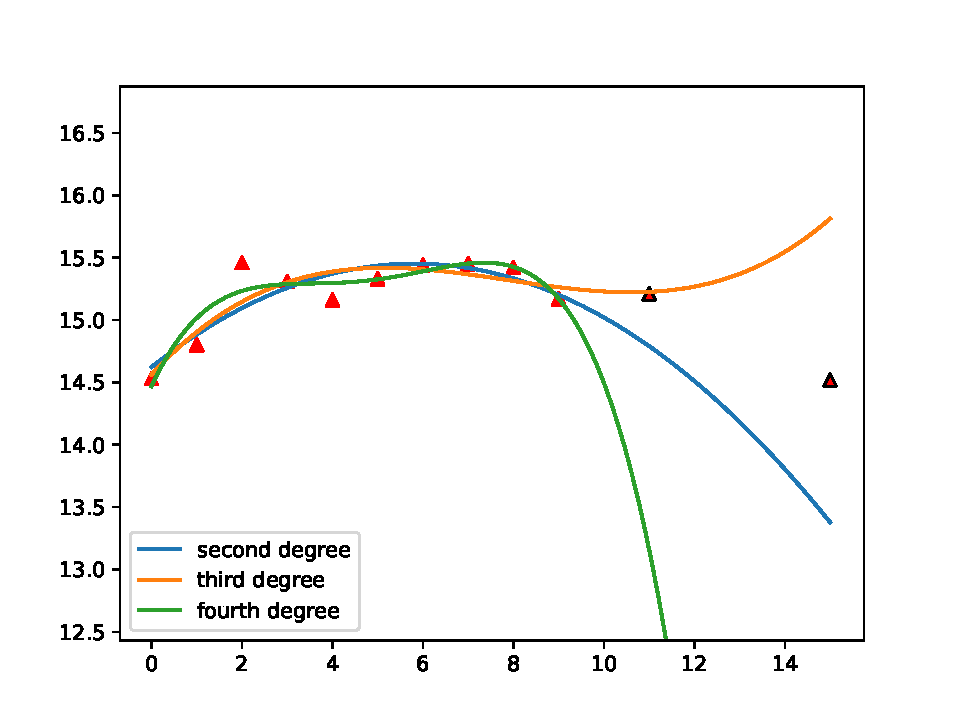
\includegraphics[width=0.8\linewidth]{images/figure7_ote.pdf}
    \centering
     \caption{Οι τιμές της μετοχής και η εκτίμησή τους}
    \label{fig:fig7ote}
\end{figure}

\begin{table}[h!]
\centering
\begin{tabular}{c c| c c c}
    & & \multicolumn{3}{c}{Πολυώνυμα} \\
   Ημέρα & Πραγματική τιμή & Δευτεροβάθμιο & Τριτοβάθμιο & Τεταρτοβάθμιο \\
   11 (21-2) & 15.21 & 14.7904242 & 15.2253333 & 13.1624242 \\
   15 (28-2) & 14.52 & 13.3785455 & 15.812 & -5.3955245 \\
\end{tabular}
\caption{Οι προβλέψεις τιμών για τις δύο συνεδριάσεις}
\label{fig:table7c}
\end{table}

\begin{table}[h!]
\centering
\begin{tabular}{c c c c}
    & \multicolumn{3}{c}{Πολυώνυμα} \\
   Ημέρες & Δευτεροβάθμιο & Τριτοβάθμιο & Τεταρτοβάθμιο \\
   0-9 & 0.1072242 & 0.1091515 & 0.0726247 \\
   11 (21-2) & 0.4195758 & 0.0153333 & 2.0475758 \\
   15 (28-2) & 1.1414545 & 1.292 & 19.9155245 \\
\end{tabular}
\caption{Σφάλματα των προσεγγίσεων}
\label{fig:table7d}
\end{table}

Και σε αυτή την περίπτωση τα πολυώνυμα προσεγγίζουν αρκετά καλά τις τιμές της μετοχής για ημέρες 0 έως 9. Την ενδέκατη ημέρα (21η Φεβρουαρίου 2023) το πολυώνυμο τρίτου βαθμού εκτιμά με ακρίβεια λεπτού του ευρώ την τιμή. Τα πράγματα όμως αλλάζουν την δέκατη πέμπτη ημέρα (28η Φεβρουαρίου 2023), όποτε κανένα πολυώνυμο δεν εκτιμά με καλή ακρίβεια την τιμή και συγκεκριμένα το τεταρτοβάθμιο πολυώνυμο μάς επιστρέφει αρνητική τιμή! 

\subsection{Συμπεράσματα}

Έχοντας στη διάθεσή μας τα αποτελέσματα παρατηρούμε ότι οι εκτιμήσεις για την τιμή μιας μετοχής δεν συνάδουν πάντα με την πραγματικότητα. Πολλές φορές μάλιστα διαφορετικές μέθοδοι προσέγγισης επιστρέφουν αποτελέσματα με μεγάλη απόκλιση μεταξύ τους. Τα γενικά συμπεράσματα είναι ότι δεν μπορούμε να βασίζουμε τις επενδύσεις μας σε πολυωνυμικές προσεγγίσεις (τουλάχιστον όχι αποκλειστικά σε αυτές). Η αγορά μετοχών χαρακτηρίζεται από μεγάλη πολυπλοκότητα και υπάρχουν πολλοί συντελεστές που καθορίζουν τη λειτουργία της.

\begin{thebibliography}{2}

\lt
\bibitem{sauer}Timothy Sauer. \gt \emph{Αριθμητική Ανάλυση, Τρίτη Έκδοση}. 
\bibitem{tefas}Αναστάσιος Τέφας. \emph{Σημειώσεις του μαθήματος Αριθμητική Ανάλυση}. Τμήμα Πληροφορικής ΑΠΘ, 2023-2024.
    
\end{thebibliography}

\end{document}